Instead of relying upon a source owned by Alice, which could be tapped by Eve, a source
emits pairs of spin-$1/2$ particles ($|{\bm{\uparrow}}\rangle$ or $|{\bm{\downarrow}}\rangle$) in singlet states
\begin{center}
    $\phi = \dfrac{(|{\bm{\uparrow}\bm{\downarrow}}\rangle + |{\bm{\downarrow}\bm{\uparrow}}\rangle)}{\sqrt{2}}$
\end{center}
that Alice and Bob share.
In state $|{\bm{\uparrow}\bm{\downarrow}}\rangle$, 
particle A has an $\bm{\uparrow}$ spin and B a $\bm{\downarrow}$ spin, 
whereas in state $|{\bm{\downarrow}\bm{\uparrow}}\rangle$ particle A
has a $\bm{\downarrow}$ spin and B an $\bm{\uparrow}$ spin. 
The well-defined combined state of both particles and the unknown spin of either particle 
is called the superposition of states. In other words, it is known that one particle is spinning up 
and the other is spinning down, but it is impossible to tell which particle is which.
Both Alice and Bob randomly pick one of the three axes-bases in which to measure the
incoming particles, that can be mathematically represented as vectors
$a_{i}$ and $b_{j}$, respectively $(i, j = 1, 2, 3)$.
Assuming the particles are traveling along the z axis, the vectors $a_{i}$ and $b_{j}$ are
located in the $x-y$ plane, perpendicular to the trajectory of the particles.
By using the vertical x axis from which to measure the angles, the vectors
$a_{i}$ and $b_{j}$ can be described by 
$\phi^{a}_{1}= \ang{0}$, $\phi^{a}_{2}= \ang{45}$ and $\phi^{a}_{3}= \ang{90}$ and 
$\phi^{b}_{1}= \ang{45}$, $\phi^{b}_{2}= \ang{90}$ and $\phi^{b}_{3}= \ang{135}$: 
the orientation of Alice and Bob's analyzers, respectively. 
Each measurement can yield two results, $+1$ (spin $\bm{\uparrow}$) and $-1$ (spin $\bm{\downarrow}$), 
potentially revealing one bit of information.
\begin{figure}[!h]
\centering
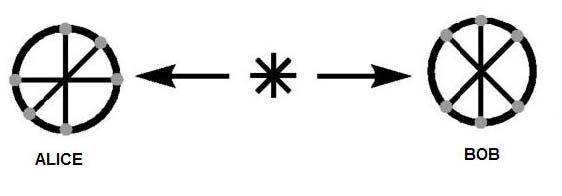
\includegraphics[width=\textwidth,height=\textheight,keepaspectratio]{6.png}
\caption{Possible basis-axis orientations for Alice and Bob}
\label{fig6}
\end{figure}
Thus, there is a $1/3$ probability that Alice and Bob’s bases will be compatible. For
example, if Alice and Bob chose a compatible basis, and Alice measured a spin $\bm{\uparrow}$ particle,
the quantum state of the system would collapse into state $|{\bm{\uparrow}\bm{\downarrow}}\rangle$, and the probability of Bob
measuring a spin $\bm{\downarrow}$ particle would be $100\%$. In that respect, if Alice observes a spin $\bm{\downarrow}$
particle, Bob will detect a spin $\bm{\uparrow}$ particle with a $100\%$ probability. However, if Alice and
Bob measured the spins in incompatible bases, we cannot be that certain about the
outcome. If Alice measures the particles in one basis, Bob's measurement outcome in a
non-compatible basis will be random. For example, if Alice detects a spin $\bm{\uparrow}$ particle in the $a_{2}$ basis 
and Bob measures in the incompatible $b_{2}$ basis, there exists an equal $50\%$ probability of detecting either 
a spin $\bm{\uparrow}$ or a spin $\bm{\downarrow}$ particle.
Due to entanglement, it is implied that Bob's particle somehow ``knows" how Alice's particle was measured 
and orients itself accordingly. There seems to exist some form of action or
connection at a distance, informing Bob's particle about the basis Alice used, so that his
particle can ``decide" whether or not it should complement Alice's measurement in the same
basis, or pick a random orientation, if incompatible bases are chosen.
So, if Alice and Bob choose compatible bases, their measurement results will be anti-correlated 
(Bob's particle will have spin $\bm{\uparrow}$, and Alice's will have spin $\bm{\downarrow}$). 
And if they choose incompatible bases, the {\it sifting} takes place, where they must publicly
announce which bases the particles were measured in order to discard the corresponding
bits (of differing bases) without needing to reveal them (that is: the outcomes of their measurements).
The remaining ``sifted key" shrinks down to $30\%$ of its original size (on average). 
Within the ``sifted key", the spin $\bm{\uparrow}$ and spin $\bm{\downarrow}$ states of the particles 
usually correspond to bit values $0$ and $1$.
But, how are we secure against Eve gaining any information about the key?
Until a measurement is made, the states of the particles are not yet collapsed.
So, trying to gain information about the system without making a measurement is impossible because 
no information yet ``exists". For example, let's say both Alice and Bob choose to measure a particle
in the $\ang{45}$ basis ($a_{2}$ and $b_{1}$, respectively), and Alice detects a
spin $\bm{\uparrow}$ particle, then Bob must definitely detect a spin $\bm{\downarrow}$ particle. 
If Bob does not, it might mean that Eve has tapped on the connection. If Eve is indeed trying to intercept, she must
choose a basis in which to measure her particle. If she detects the particle in her basis, it
means that she has measured it, therefore destroying it. If Eve's basis is different from Alice and Bob's, 
she will get a random measurement result. She will then have to recreate her detected particle 
(usually in the basis of her measurement) and send it to Bob.
After such an intervention, the orientation upon measurement (Bob's received particle) will be
random. If he measures an orientation that does not correlate to Alice's result (as Eve did), he will get an error.
Contrary to BB84's four states, the reason E91 utilizes six is so that an eavesdropper can be
detected without having to leak out information about his key, as happens in the former protocol.\\
The quantity
\begin{center}
  $E(a_{i}, b_{j}) = P_{++}(a_{i}, b_{j}) + P_{--}(a_{i}, b_{j}) - P_{+-}(a_{i}, b_{j}) - P_{-+}(a_{i}, b_{j})$
\end{center}
is the correlation coefficient of Alice and Bob's $a_{i}$ and $b_{j}$ measurements.
Where $P_{\pm\pm}(a_{i}, b_{j})$ denotes the probability of obtaining $\pm1$ along $a_{i}$ and $\pm1$ along $b_{j}$
(with $\pm1$ meaning spin $\bm{\uparrow}$ or spin $\bm{\downarrow}$). As mentioned earlier, and as predicted by quantum entanglement, 
the two pairs of analyzers of the same orientation ($a_{2}$, $b_{1}$ and $a_{3}$, $b_{2}$) give a value of
$E(a_{2}, b_{1}) = E(a_{3}, b_{2}) = -1$, which hints anti-correlation of the results obtained by Alice and Bob.
Now, one can define a quantity $S$, which is the sum of all correlation coefficients for which Alice and Bob used analyzers
of different orientations (incompatible bases):
\begin{center}
$S = E(a_{1}, b_{1}) - E(a_{1}, b_{3}) + E(a_{3}, b_{1}) + E(a_{3}, b_{3})$
\end{center}
Bell, using local realism, proved that $S\leq2$. However, quantum mechanics gives that $S = 2\sqrt{2}$.
This simply means that if the states are truly entangled, the rules of local realism are
defied and Bell's theorem is violated. Therefore, by publicly announcing the values Alice
and Bob measured in an incompatible basis, they can figure out a value for $S$. Therefore,
after the transmission has taken place, Alice and Bob can publicly announce the
orientations of the analyzers they have chosen for each particular measurement.
Specifically, they divide the measurements into two groups:
\begin{enumerate}
	\item A group for which they used different orientation of analyzers
	\item A group for which they used the same orientation of their analyzers.
\end{enumerate}
Subsequently, Alice and Bob publicly reveal the results obtained within the first group of measurements only, 
which allows them to establish the value of $S$. If the particles were not disturbed by Eve, or anything else, 
their expected value is $2\sqrt{2}$ and they can rest assured
that the values they measured in a compatible basis are anti-correlated and that their
{\it sifted key} is secure. It should generally not be forgotten that even if the possibility of an
eavesdropper is eliminated, the sifted key may contain other, system-related errors.
So, anything different to anti-correlation indicates an error occurrence in the system. 

A portion of detected errors is referred to as the Quantum Bit Error Rate (QBER). 
The QBER is calculated by dividing the number of errors by sample size and multiplying by $100\%$ 
and it is an indication of the efficiency of the system. In general, an error rate that exceeds 
approximately $15\%$ serves as a good indication that some malicious Eve is present.
Assuming that the possibility of Eve was eliminated, Alice and Bob proceed onto refining
their keys through error correction and privacy amplification (which are both classical
algorithms, used for further securing the final key). 
Finally, after error-correction has been applied to the sifted key, Alice and Bob may use 
the resulting key to safely communicate.
